% This must be in the first 5 lines to tell arXiv to use pdfLaTeX, which is strongly recommended.
\pdfoutput=1
% In particular, the hyperref package requires pdfLaTeX in order to break URLs across lines.

\documentclass[11pt]{article}

% Remove the "review" option to generate the final version.
% \usepackage[review]{ACL2023}
\usepackage{ACL2023}


% Standard package includes
\usepackage{times}
\usepackage{latexsym}
\usepackage{graphicx} % For including images
\usepackage{amsmath,amssymb} % Mathematical symbols and environments
\usepackage[export]{adjustbox}
\usepackage{tabularx}
\usepackage{pgfplots}
%\usepackage{todonotes}


% For proper rendering and hyphenation of words containing Latin characters (including in bib files)
\usepackage[T1]{fontenc}
% For Vietnamese characters
% \usepackage[T5]{fontenc}
% See https://www.latex-project.org/help/documentation/encguide.pdf for other character sets

% This assumes your files are encoded as UTF8
\usepackage[utf8]{inputenc}

% This is not strictly necessary, and may be commented out.
% However, it will improve the layout of the manuscript,
% and will typically save some space.
\usepackage{microtype}
\usepackage{subcaption}


% This is also not strictly necessary, and may be commented out.
% However, it will improve the aesthetics of text in
% the typewriter font.
\usepackage{inconsolata}


\definecolor{plt_blue}{RGB}{31, 119, 180}
\definecolor{plt_orange}{RGB}{255, 127, 14}
\definecolor{plt_green}{RGB}{44, 160, 44}
\definecolor{plt_red}{RGB}{214, 39, 40}
\definecolor{plt_purple}{RGB}{148, 103, 189}
\definecolor{plt_cyan}{RGB}{0,157,174}
\definecolor{plt_pink}{RGB}{227,119,194}


% If the title and author information does not fit in the area allocated, uncomment the following
%
%\setlength\titlebox{<dim>}
%
% and set <dim> to something 5cm or larger.

\title{
Comparative Study of Classical and Neural Retrieval Methods for FANDOM Wikis
}

\author{
Aaron Kutzer \and Florian M. Müller \and Till Dirschnabel  \and \\
{\bf Tommy Nguyen} \and {\bf Zhìwēi Zhān} \and {\bf Anja Reusch} \and {\bf Julius Gonsior} \\
Dresden University of Technology \\ Dresden, Germany
}


\begin{document}
\maketitle
\begin{abstract}
This paper investigates the effectiveness of traditional information retrieval methods and the neural retrieval method ColBERT in the context of locating relevant passages within fandom wikis. To facilitate this study, we developed a new dataset called FANDOM-QA, consisting of query and answering passage pairs. Additionally, we provide a novel analysis of the operational mechanisms employed by ColBERT, shedding light on its functioning and capabilities.
\end{abstract}


\section{Introduction}
%Maybe a small introduction about our task and the field of information retrieval (especially classical retrieval vs neural retrieval)?
Natural language processing has developed at an astonishing rate in recent years. 
An important task of natural language processing is information retrieval which consists of finding relevant information to answer a given questions. Classical retrieval methods do not have semantic understanding of language \cite{hambarde2023information}, severely limiting the information retrieval, this changed with neural retrieval. \\
Our research consists of implementing a semantic retrieval system performing extractive question answering on fandom wikis sourced from \href{https://www.fandom.com/}{fandom.com}. Both classical and neural retrieval methods were tested on their effectiveness for this task. For this, we first extracted and cleaned publicly available fandom wiki exports and secondly generated our own training and validation datasets, which were used for training and evaluation of the retrieval methods.
Furthermore, this paper discusses and evaluates optimisation methods for training datasets and hyperparameters and visualization methods to gain a better understanding of ColBERT.
We start by introducing the datasets and their construction (Chapter~\ref{chap:datasets}), then we explain our retrieval methods and their training (Chapter~\ref{chap:retrieval}). In Chapter~\ref{chap:results}, we present the results obtained in terms of metrics, hyperparameters and multi-stage fine-tuning.
Finally in Chapter~\ref{chap:understanding}, we introduce visualisation methods to better understand Colbert and find the answer in the extracted passage, and discuss the observations made.

\section{Datasets}
\label{chap:datasets}
For training and validation of the retrieval system, we utilized two datasets: the publicly available MS MARCOv2 \cite{bajaj2018ms} dataset and our custom dataset, FANDOM-QA. \\
The MS MARCO dataset was used in the first stage of multi-stage fine-tuning in our neural retrieval models and to validate our implementation against the original implementation, while the FANDOM-QA dataset was later used in the second stage of multi-stage fine-tuning. In this second stage, either the entire dataset or a subset of the dataset corresponding to a particular wiki were used. \\
Figure \ref{qword-dist} and \ref{table1} provide information about the size of the datasets and the distribution of the fandom wikis in the FANDOM-QA dataset.

\begin{figure}
    \centering
    \begin{tikzpicture}
    \small
    \begin{axis}[
        width=7.7cm,
        height=6cm,
        ylabel={Percentage},
        xlabel={},
        xtick=data,
        xticklabel style={rotate=30, anchor=north, yshift=-0.12cm, xshift=-0.15cm},
        xticklabels={Marvel, Star Wars, Harry Potter, Elder Scrolls},
        enlarge x limits={abs=0.6},
        ymin=0,
        ymax=85,
        yticklabel={\pgfmathprintnumber{\tick}\%},
        legend style={at={(0.75,0.9)},
            anchor=north,legend columns=-1},
        ybar=0pt,
        bar width=0.4cm,
        nodes near coords,
        nodes near coords style={font=\scriptsize},
        every node near coord/.append style={rotate=90, anchor=west},
        legend style={yshift=1em, xshift=-1em}, % Reduce the padding between legend and plot area
        legend cell align=right top, % Align legend items horizontally
    ]
    
    \addplot[fill=plt_blue,draw=plt_blue] coordinates {
        (0, 1.8)
        (1, 70.4)
        (2, 7.4)
        (3, 20.4)
    };
    
    \addplot[fill=plt_orange,draw=plt_orange] coordinates {
        (0, 8.8)
        (1, 12.8)
        (2, 36.1)
        (3, 42.3)
    };
    \addlegendentry{Passages}
    \addlegendentry{Queries}
    
    \end{axis}
    \end{tikzpicture}
    \caption{Percentage of Passages and Queries of each Wiki in the FANDOM-QA dataset}
    \label{qword-dist}
\end{figure}
\setlength{\textfloatsep}{8pt} 



\subsection{FANDOM-QA}
The FANDOM-QA dataset was constructed by extracting all passages from the specific fandom wikis: \href{https://dc.fandom.com}{DC Comics}, \href{https://elderscrolls.fandom.com}{Elder Scrolls}, \href{https://harrypotter.fandom.com}{Harry Potter}, \href{https://marvel.fandom.com}{Marvel}, \href{https://starwars.fandom.com}{Star Wars}, and \href{https://witcher.fandom.com}{The Witcher} using the the assistance of the \textit{wikiextractor} tool \cite{Wikiextractor2015}. \\
Next, we generated positive and negative queries for all passages. Positive questions are designed to have answers that can be found in the passage, while negative questions cannot be answered using the information in the passage. To expedite this process, we utilized publicly available GPT-frontends using the \textit{gpt4free}\footnote{\url{https://github.com/xtekky/gpt4free}} repository. \\
To ensure effective evaluation of our neural retrieval method, we partitioned the dataset into two subsets: training and validation. The training subset constituted 89\% of the data, while the validation contained 11\%. \\
It is important to note that these steps were performed separately for each wiki, and the resulting datasets were then merged to create the final FANDOM-QA dataset. This ensured that our models could be trained and evaluated on specific fandom wikis or all collected wikis, while preventing information leakage between the training and evaluation datasets. 
We also wanted to evaluate our model on a wiki on which the model had not been trained. We used the Witcher dataset for this, and consequently did not include it in the Fandom-QA dataset. A few random samples of the dataset can be found in Figure \ref{tab:fandom-qa}.\\
We observed some problems with query generation using GPT. One obstacle was observed during training in the second stage of the multi-stage fine-tuning. 
A high proportion of the words in the negative query also appeared in the passage. To our surprise, this led to a drastic decrease in the performance of our model, possibly due to the loss function we used. % in the second stage of multi-stage fine-tuning, possibly due to the loss function we used.
To overcome this obstacle, we shuffled the negative queries in the FANDOM-QA training dataset to obtain a dataset where the positive and negative queries for a passage are more diverse.

% A high proportion of the words contained in the negative query also occurred in the passage. To our surprise, this led to a drastic decrease in performance of our model in the second stage of multi-stage fine-tuning. A possible reason might be that cross-entropy that we used also tried to minimise the similarity between the passage and the negative query. This problem was solved by shuffling the negative queries.
%To further enhance the dataset's quality, a small human-verified dataset was manually created for the Harry Potter, Elder Scrolls, and The Witcher fandoms containing 2,870 queries. This human dataset underwent careful scrutiny to ensure its correctness. The intention behind this step was to train the final model using the human dataset, thereby improving its performance further.\\



\section{Retrieval Methods}
\label{chap:retrieval}
\subsection{Classical Retrieval Methods}
We used Term Frequency - Inverse Document Frequency (TF-IDF), a classic retrieval method, as a baseline model for comparison and for the re-ranking retrieval method described in Chapter~\ref{chap:retrieval}. TF-IDF quantifies the importance of terms in a collection of documents by determining the frequency of a term (TF) within a document and adjusting it based on the inverse document frequency (IDF) across the collection. Thus, terms that occur more frequently within a particular document, but are relatively rare across the collection, are given high weights. By representing the query and the passages as vectors containing a TF-IDF value for each term that occurs in the entire corpus, the passages can be ranked using cosine similarity. However, TF-IDF has significant limitations. It assumes that the importance of a term depends solely on its frequency and treats each term as an independent entity, ignoring contextual factors such as the order or proximity of terms within a document, as well as synonyms. As a result, TF-IDF cannot capture semantic meaning, a problem that neural approaches seek to overcome.

\subsection{Neural Retrieval Methods}
For our neural retrieval approach, we adopted the ColBERT \cite{khattab2020ColBERT} model, which utilizes Transformer models to generate vector embeddings for word tokens in a text sequence. These embeddings capture the contextual information of the tokens within the sequence and are then used to calculate the similarity between two sequences.

\subsubsection{ColBERT Model}
The ColBERT model takes a query and a document passage as input. These strings are then tokenized using the Transformer model's associated tokenizer, resulting in sequences of query tokens ($q = q_1q_2\dots q_m$) and document tokens ($d = d_1d_2\dots d_n$). Next we prepend a \texttt{[CLS]} token at the beginning and append a \texttt{[SEP]} token at the end of both sequences and add either a \texttt{[Q]} or \texttt{[D]} token after the \texttt{[CLS]} token to encode the input sequence type (query or document/passage). The query and document sequences are constrained to maximum lengths of $N_q$ and $N_d$ tokens, respectively. If the query is shorter than $N_q$ tokens, we pad the sequence with \texttt{[MASK]} tokens until it reaches length $N_q$. The document sequence will not be padded if shorter than $N_d$ and will be of length $L_d = min(n + 3, N_d)$. Thus, the input sequences for the ColBERT model are as follows: \\ $q = \texttt{[CLS]}\texttt{[Q]}q_1q_2 \dots q_m\texttt{[SEP]}\texttt{[MASK]}\dots\texttt{[MASK]}$ and $d = \texttt{[CLS]}\texttt{[D]}d_1d_2 \dots d_{L_d-3}\texttt{[SEP]}$, respectively. These tokenized sequences are then passed through a Transformer model's Encoder, with experiments conducted using both BERT \cite{devlin2019bert} and RoBERTa \cite{liu2019roberta} architectures. The resulting output is a sequence $E = E_1E_2 \dots E_k$ of high-dimensional vectors, where $k$ corresponds to $N_q$ or $L_d$, depending on the sequence being processed. These vectors are subsequently mapped to a lower dimensionality $d$ using a linear transformation. To calculate the similarity between the query and document sequences, we employ the \textit{sum of maximum similarity} function, as presented by the authors of ColBERT. However, instead of using the sum, we use the mean to obtain a more interpretable similarity score. The function is computed as follows:
\[ S(q,d) := \frac{1}{N_q} \sum_{i=1}^{N_q} \max_{j = 1, \dots, L_d} sim(E_{q_i}, E_{d_j})
\]
We evaluate similarity between embedding vectors using both cosine similarity and negated squared $L_2$-norm.
Originally, the vectors were normalized before applying these similarity measures. However, we also experimented with $L_2$-norm without normalization of the embedding vectors.
The formulas for the similarity measures can be found in the Appendix~\ref{appendix:similarity}. 

\subsubsection{ColBERT Training}
During the training the BERT/RoBERTa encoder is fine-tuned and the last linear projection and the additional \texttt{[Q]}/\texttt{[D]} tokens are learned from scratch. For training on the MS MARCO dataset, the model receives batches of tuples in the form $\langle q_i^+, d_i^+, d_{i, 1}^-, \dots, d_{i, 9}^-\rangle$. Here, $d_i^+$ represents the answer passage for the query $q_i^+$, and the passages $d_{i, l}^-$ do not contain the answer. 
The FANDOM-QA dataset contains negative queries for a passage, rather than providing negative passages for a query.
%that were generated to not be answered by a passage. 
So when training on our FANDOM-QA dataset, the model receives batches of tuples in the form $\langle q_i^+, q_i^-, d_i^+\rangle$, where $q_i^+$ is answered by $d_i^+$ while $q_i^-$ is not. Despite the differences in data format, the training objective remains the same: maximizing the similarity between the answering query/passage pairs relative to the other given passages. The loss is calculated using the cross-entropy loss and is defined as follows for the MS MARCO dataset:
$$
\ell = -\frac{1}{B} \sum_{i=1}^{B} \log \frac{e^{N_q S(q_i^+, d_i^+)}}{e^{N_q S(q_i^+, d_i^+)} + \sum_{j=1}^{9}{e^{N_q S(q_i^+, d_{i, j}^-)}}}
$$
For the FANDOM-QA dataset, the loss function becomes:
$$
\ell = -\frac{1}{B} \sum_{i=1}^{B} \log \frac{e^{N_q S(q_i^+, d_i^+)}}{e^{N_q S(q_i^+, d_i^+)} + e^{N_q S(q_i^-, d_i^+)}}
$$
Sadly, it was observed during our experiments that it is necessary to manually scale the similarity scores by a factor of $N_q$ in order to achieve better convergence during training (so we actually use the sum of maximum similarity for training). The reason behind this requirement is likely attributed to the range of cosine similarity scores, which typically fall between -1 and 1. Even in an ideal scenario where predicted similarities take the form of $\langle 1, -1, \dots, -1\rangle$, applying the softmax function yields probabilities such as $\langle 0.451, 0.061, \dots, 0.061\rangle$, which is similar to using extremly aggressive label smoothing \cite{szegedy2015rethinking}. Unfortunately, we have not been successful in devising an alternative loss function to address this limitation. \\
We conducted experiments using Mean Squared Error (MSE) loss in combination with cosine similarity. In this setup, the target for the loss function was set to 1 for the pairs $\langle q, d^+\rangle$ representing answering passages. Conversely, for the pairs $\langle q, d^-\rangle$ representing not answering passages, we enforced orthogonality by aiming for a cosine similarity of 0. However, this approach yielded inferior performance, as demonstrated in the subsequent analysis.

\subsubsection{Retrieval with ColBERT} \label{chap:retrieval}
Due to the computational cost associated with calculating the similarity between a given query and all passages, we adopt the two methods from the original ColBERT paper: \textit{re-ranking} and \textit{end-to-end retrieval}. In the \textit{re-ranking} approach, we employ a classical retrieval algorithm (in our case TF-IDF) to retrieve the top-$k$ passages for a query. Subsequently, ColBERT is used to re-rank these $k$ documents based on their similarity scores. On the other hand, \textit{end-to-end retrieval} exclusively utilizes ColBERT. For a given query, we search for the top-$\hat{k}$ most similar document embedding vectors for each of the $N_q$ query embedding vectors. In the original work this was done using the vector search framework \texttt{faiss}, however due to time limitation we used a simple precomputed document embedding matrix and exhaustively calculated the similarities. We retrieve the associated documents ($\leq \hat{k}N_q$ unique documents) and calculate the similarity between the query and these documents. Finally, we return the top-$k$ documents. 
The validation of our implementation with the original implementation can be found in the Appendix \ref{appendix:validationimplementation}.

\section{Results}
\label{chap:results}
This chapter showcases the results of our conducted experiments on ColBERT with the aim of
(1) assessing the significance of various hyperparameters in relation to the retrieval performance, and
(2) evaluating the comparative advantages of training the model using all fandoms versus specific ones, as well as its ability to generalize to unseen wikis.
To address task (1), we conducted an extensive experimental phase of hyperparameter optimization. %(Appendix ~\ref{appendix:hyperparameters}). 
The performance of each model was evaluated using selected metrics (Chapter~\ref{chap:metrics}). 
Subsequently, we fine-tuned the model with the best hyperparameter settings on our FANDOM-QA dataset and the Harry Potter dataset  (Chapter~\ref{chap:fine-tuning}).

\subsection{Metrics}
\label{chap:metrics}
We placed emphasis on computing Recall@k and MRR@k, which are two commonly used model evaluation metrics that are crucial for assessing the information retrieval capability and ranking accuracy of a model and are also used in the official ColBERT paper, allowing for comparison. 
In both cases, @k represents the truncation value, beyond which a passage is deemed a false negative or, in the case of MRR, assigned a reciprocal rank of 0. 
\[
\text{Recall@}k = \frac{TP@k}{P} \]
\[
\text{MRR@}k = \frac{1}{|Q|} \sum_{i=1}^{|Q|} r
\begin{cases}
r = \frac{1}{\text{rank}_i} & \text{if } \text{rank}_i \leq k \\
r =  0 & \text{otherwise}
\end{cases}
\]
In the MS MARCOv2 dataset, it is important to note that a single query $q_i^+$ can have multiple relevant documents $d_{i,j}^+$. Therefore, we opted to use recall instead of accuracy to account for this variability. When calculating MRR@k, we consider the rank of the highest-ranked relevant document $d_{i,l}^+$. In contrast, the FANDOM-QA dataset consists of a single answering passage per query, rendering the calculation of accuracy or recall indistinguishable in this context, so we sticked with recall for its validation.

\subsection{Hyperparameter Search} \label{hparameter-chapter}

To determine the optimal hyperparameter configuration for our ColBERT model, we conducted a manual sequential optimization strategy. We systematically changed specific hyperparameters while keeping others constant. During the search, all models  were trained on MS MARCOv2. Additional details regarding the training process can be found in Appendix~\ref{appendix:constsettings}. \\
The investigated hyperparameters included the embedding dimension ($d$), with values of 8, 16, 24, 32, 64, and 128. We compared three similarity calculation methods: cosine similarity, $L2$ distance, and normalized $L2$ distance similarity. We tested training with either cross-entropy or mean squared error loss. The impact of varying the number of query embedding vectors ($N_q$) was also explored, with values of 32 and 64. Furthermore, the performance of BERT and RoBERTa architectures as backbone models was compared. Additionally, the influence of reducing the ratio $\hat{k} = \frac{k}{\lambda}$ on the end-to-end retrieval performance was examined. Detailed results for each hyperparameter configuration can be found in Figure \ref{hparameter-end2end} for end-to-end retrieval and Figure \ref{hparameter-rerank} for re-ranking.\\
The evaluation results indicate that the original configuration used in the ColBERT paper is mostly optimal in terms of hyperparameter settings. However, a slight improvement in performance was observed with an increased value of $N_q$. The best performing setting determined by our search is as follows: 128 embedding dimensions, cosine similarity, cross-entropy loss function, BERT as the backbone model, 64 embedding query vectors, and $\hat{k} = k / 2$. Interestingly, decreasing the value of $\hat{k}$ did not significantly impact the retrieval process, particularly for the top 10 results which receive the most focus in our retrieval process, as users are less likely to explore lower-ranked results. Therefore, we set $\hat{k} = k / 5$ to reduce the number of passages to rank and consequently save inference time. \\
Interestingly, during the evaluation phase, the model using a BERT backbone consistently outperformed the model with a RoBERTa backbone, despite RoBERTa being a superior trained BERT model. To strengthen this observation, we conducted tests on RoBERTa with various hyperparameter settings. However, all of these settings resulted in poorer performance compared to the BERT backbone. Regrettably, we are unable to explain the underlying cause of this behavior.


\subsection{Multi-Stage Fine-Tuning}
\label{chap:fine-tuning}
After identifying the best hyperparameters in Chapter~\ref{hparameter-chapter}, we conducted a Multi-Stage Fine-Tuning process to train a robust retrieval model for our FANDOM-QA dataset. In the first stage, we preadapted ColBERT on MS MARCOv2, as the dataset provides fundamental semantic knowledge for ColBERT in retrieving correct answers to queries. In the second stage, we performed fine-tuning seperatly on the FANDOM-QA and Harry Potter datasets. We trained those two models separatly, since we wanted to test if it is necessary to train a model for each wiki seperatly or if a more general model would be similarly capable. 
We should mention that we not only trained models with 128-dimensional embeddings but also with 24-dimensional embeddings. We made this decission, since choosing 24 dimensions reduces the required storage for the precomputed document embeddings by a factor of 5, while maintaining reasonable retrieval performance. Additionally, we increased $N_q$ to 48 to enhance performance with smaller additional computational cost compared to 64. During this training, a learning rate of 3e-6 and a batch size ($B$) of 42 were employed for improved stability. \\
The results for the first stage, along with a comparison to the classical retrieval method TF-IDF, can be seen in Figure \ref{final-models}. It is evident that all ColBERT settings perform significantly better than TF-IDF, with 128-dimensional embeddings and end-to-end retrieval yielding the best recall. Interestingly, the re-rank method outperforms end-to-end retrieval for 24-dimensional embeddings. Due to time limitations, we were unable to investigate the cause of this behavior further, but it presents an intriguing avenue for future research.
\begin{figure}
    \centering
    \caption{Retrieval Performance on MS MARCOv2 (Eval)}
    \label{final-models} 
    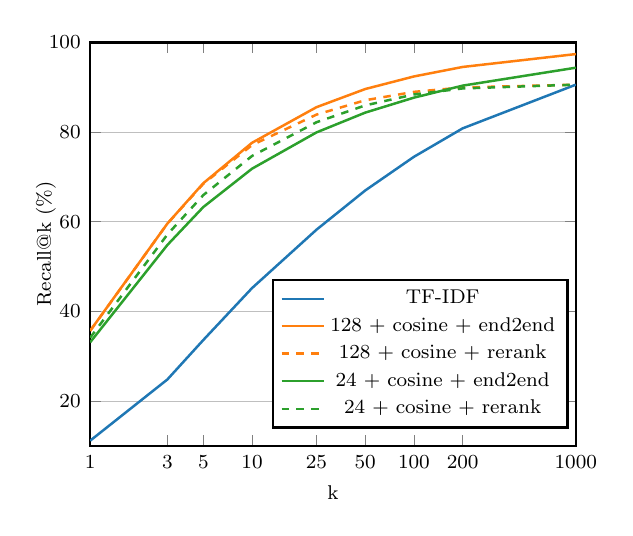
\begin{tikzpicture}[scale = 0.9]
    \begin{semilogxaxis}[
        xlabel = {k},
        ylabel={Recall@k (\%)},
        xmin = 1, xmax = 1000,
        ymin = 10, ymax = 100,
        xtick=data,
        xticklabels={1,3,5,10,25,50,100,200,1000},
        legend pos = south east,
        line width = 1pt,
        ymajorgrids = true,
        font=\footnotesize,
        ylabel style={yshift=-1em}, % Reduce the padding between y-axis label and y-axis
        legend style={yshift=0.2em, xshift=0.3em}, % Reduce the padding between legend and plot area
        ]
    
    \addplot[color=plt_blue, line width=1pt]
        coordinates {
        (1, 11.154)(3, 24.812)(5, 33.609)(10, 45.194)(25, 58.212)(50, 66.963)(100, 74.479)(200, 80.823)(1000, 90.566)
    }; \addlegendentry{TF-IDF}
    
    \addplot[color=plt_orange, line width=1pt]
        coordinates {
        (1, 35.683)(3, 59.577)(5, 68.586)(10, 77.607)(25, 85.544)(50, 89.592)(100, 92.401)(200, 94.519)(1000, 97.393)
    }; \addlegendentry{128 + cosine + end2end }
    
    \addplot[color=plt_orange, line width=1pt, dashed]
        coordinates {
        (1, 35.649)(3, 59.572)(5, 68.45)(10, 77.088)(25, 83.888)(50, 87.094)(100, 88.964)(200, 89.95)(1000, 90.566)
    }; \addlegendentry{128 + cosine + rerank}
    
    \addplot[color=plt_green, line width=1pt]
        coordinates {
        (1, 33.101)(3, 54.81)(5, 63.27)(10, 71.8267)(25, 79.916)(50, 84.331)(100, 87.674)(200, 90.353)(1000, 94.352)
    }; \addlegendentry{24 + cosine + end2end}
    
    \addplot[color=plt_green, line width=1pt, dashed]
        coordinates {
        (1, 34.12)(3, 57.14)(5, 65.936)(10, 74.664)(25, 82.186)(50, 85.944)(100, 88.379)(200, 89.728)(1000, 90.566)
    }; \addlegendentry{24 + cosine + rerank}
    
    \end{semilogxaxis}
    \end{tikzpicture}
\end{figure}
\\
The end-to-end retrieval performances of the second stage models on the Harry Potter dataset, as seen in Figure \ref{FandomQAvHP}, show similar performance between the models fine-tuned on FANDOM-QA and Harry Potter, with a slight lead observed for the FANDOM-QA model. However, when comparing these models to the preadapted model, a significant performance difference was observed. This difference could be attributed to the fine-tuned models being trained on well-formulated questions and performing on a smaller information pool, while the preadapted model dealt with more diverse and extensive topics. The fine-tuned models may have also adopted certain formulations frequently used by GPT, leading to improved performance. \\
%A further obstacle in using the GPT generated queries was observed during the training. 
%A high proportion of the words contained in the negative query also occurred in the passage. To our surprise, this led to a drastic decrease in performance of our model in the second stage of multi-stage fine-tuning. %A possible reason might be that cross-entropy that we used for training also tried to minimise the similarity between the passage and the negative query. 
%Consequently, we shuffled the negative queries among in the test dataset to obtain a dataset that does not have this problem.\\
We also evaluated the generalization capabilities of the models to unseen data, by utilizing the Witcher dataset. The results, seen in Figure \ref{FandomQAvHPonWitcher}, indicated that the more general model performed better than the model trained solely on Harry Potter. However, the performance of both models was still quite similar, suggesting again a potential flaw in the autogenerated questions generated by GPT-3, since repetitive formulation in the fine-tuned models may have led to an excessive performance in this context. \\
In conclusion, the end-to-end retrieval method is superior to the re-ranking approach. For retrieval on fandoms, a more general model (all wikis) appears to perform as well as more specialized (single wiki) models while exhibiting better generalization capability to unseen data. However, further research with more diverse data should be conducted to validate these findings.

\begin{figure}
    \centering
    \caption{End-to-End Retrieval on Harry Potter ($d=24$, $sim=\text{cosine}$)}
    \label{FandomQAvHP}
    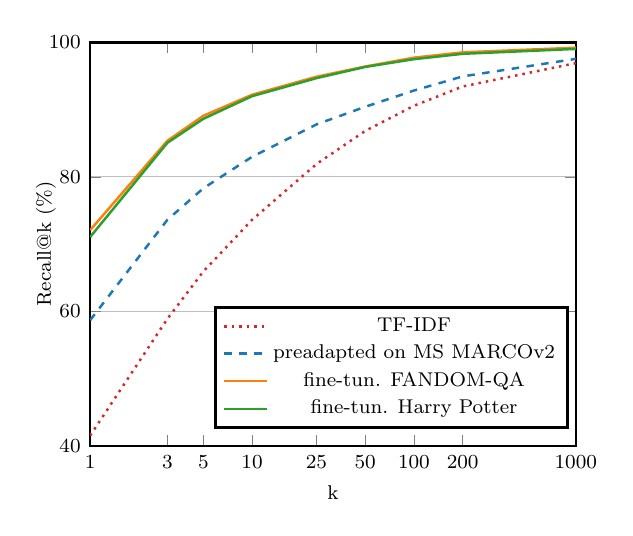
\begin{tikzpicture}[scale = 0.9]
        \begin{semilogxaxis}[
            % title = {End-to-End Retrieval on Harry Potter ($d=24$, $sim=\text{cosine}$)
            % },
            xlabel = {k},
            ylabel={Recall@k (\%)},
            xmin = 1, xmax = 1000,
            ymin = 40, ymax = 100,
            xtick=data,
            xticklabels={1,3,5,10,25,50,100,200,1000},
            legend pos = south east,
            line width = 1pt,
            ymajorgrids = true,
            font=\footnotesize,
            ylabel style={yshift=-1em}, % Reduce the padding between y-axis label and y-axis
            legend style={yshift=0.2em, xshift=0.3em}, % Reduce the padding between legend and plot area
            ]
            
            \addplot[color=plt_red, line width=1pt, dotted]
                coordinates {
                (1, 41.521)(3, 58.895)(5, 65.921)(10, 73.606)(25, 81.906)(50, 86.833)(100, 90.572)(200, 93.443)(1000, 96.912)
                }; \addlegendentry{TF-IDF}
        
            \addplot[color=plt_blue, line width=1pt, dashed]
                coordinates {
                (1, 58.69)(3, 73.62)(5, 78.3)(10, 82.98)(25, 87.8)(50, 90.42)(100, 92.84)(200, 94.94)(1000, 97.55)
                }; \addlegendentry{preadapted on MS MARCOv2}
                    
            \addplot[color=plt_orange, line width=1pt]
                coordinates {
                (1, 72.079)(3, 85.367)(5, 89.08)(10, 92.211)(25, 94.891)(50, 96.409)(100, 97.727)(200, 98.517)(1000, 99.211)
                }; \addlegendentry{fine-tun. FANDOM-QA}
                
            \addplot[color=plt_green, line width=1pt]
                coordinates {
                (1, 71.056)(3, 85.072)(5, 88.629)(10, 92.003)(25, 94.683)(50, 96.348)(100, 97.502)(200, 98.3)(1000, 99.029)
                }; \addlegendentry{fine-tun. Harry Potter}
                
        \end{semilogxaxis}
    \end{tikzpicture}
\end{figure}

\section{Model Interpretability and Explainability}
\label{chap:understanding}
As part of our study, we aimed to understand how our ColBERT model trained on MS MARCOv2 works, assess its strengths and weaknesses, and determine the location of the answer within the extracted passage.
To achieve this, we have highlighted the tokens in the passage that are highly relevant to ColBERT (Chapter~\ref{chap:visualization}), improved this highlighting method using Kernel Density Estimation to locate the answer in the passage (Chapter~\ref{chap:kde}), and summarised the main observations in (Chapter~\ref{chap:observations}). 
Finally, in Appendix~\ref{chap:context}, we conducted small-scale experiments to evaluate the respective contributions of the word embeddings and the transformer architecture to the performance of ColBERT.

\subsection{Visualization of the Relevance of Passage Tokens}
\label{chap:visualization}
To find relevant tokens in the passage, we first note that ColBERT uses the similarity between query vectors and passage vectors to determine the correct passage.
In addition, by visualising the similarity between passage tokens and query tokens as in Figure~\ref{fig:example2}, we found that the embedded query vector $E_{q_i}$ at index $i$ encodes a large part of the information of the query token $q_i$ at index $i$. The same relationship was found between the embedded passage vector $E_{d_j}$ and the passage token $d_j$.
Therefore, a passage token $d_j$ is considered relevant to ColBERT regarding a question $q$ if the associated vector $E_{d_j}$ contributes to a high similarity score $S(q, d)$.
This occurs when $E_{d_j}$ exhibits the highest similarity to one or multiple query vectors $E_{q_i}$.
We identified the ${\tilde{k}}=2$ most similar passage vectors for each query vector, although the similarity score $S$ only considers the top 1 to strike a balance between marking a sufficient amount of information without assigning high relevance to each passage token. 
The relevance $R$ of a passage token $d_j$ can be determined by the $absolute$ $count$ of query vectors that exhibit high similarity to $E_{d_j}$. 
$$
    R_{abs}(q, d_l) = |Q(q, d_l)| \text{\quad, where\quad} Q(q, d_l) = 
$$
$$
  \{E_{q_i} \mid sim(E_{q_i}, E_{d_l}) \in \underset{j = 1, \dots, L_d}{max_{\tilde{k}}} sim(E_{q_i}, E_{d_j})\}
$$
and $max_{\tilde{k}}$ returns the highest ${\tilde{k}}$ elements computed while iterating over index $j$.
%and $max_k(U) = \{a_1, a_2, \dots, a_k\}$ such that $a_1 = max(U), a_2 = max(U \setminus %\{a_1\}), \dots, a_k = max(U \setminus \{a_1, a_2, \dots, a_{k-1}\})$. 
Since the relevance of a passage vector depends not only on its frequency among the top ${\tilde{k}}$ similarities of the query vectors, but also on the value of each individual similarity, we have extended the similarity score $R_{abs}$ to $R_{acc}$:
$$
	R_{acc}(q, d_l) = \sum_{E_{q_i} \in Q(q, d_l)} sim(E_{q_i}, E_{d_l}) 
$$

\subsection{Locating the Answer in the Passage}
\label{chap:kde}
Although ColBERT identifies the passage containing the answer to the given question by comparing the passage embedding with the query embedding, in most cases the answer itself cannot be identified directly by comparing these two embeddings using $R_{abs}$ or $R_{acc}$.
In most cases, the most relevant tokens of the passage are not the answer itself, but rather the tokens that lead to the answer.
When comparing the query 'who won the football championship in 2006?' and the passage 'the football championship in the year 2006 was a great sports event that was won by italy.' of Figure~\ref{fig:example1} the highest relevance will be found in the words 'the', 'football', 'championship', '2006', 'was', 'won' and 'by' instead  of the actual answer 'italy', because the actual answer is not relevant to decide whether the question is answered in the passage. 
ColBERT was not trained to find the answer, but rather to determine whether the answer is contained within the passage.
Replacing 'italy' with any other word would have a minimal effect on the "probability" of the passage providing an answer to the question. 
Our approach to solving this problem is to use Kernel Density Estimation~\cite{kde}, by assuming that the answer is likely to be located in the areas of the passage that contain a higher concentration of relevant tokens with respect to the question.
\\
Kernel Density Estimation is a statistical method that estimates the underlying probability density function of a random variable by placing a kernel function on each data point and summing them up to create a smooth density estimate.
 %without the need to specify additional parameters beyond the choice of kernel and %smoothing factor.
Given that the queries are encoded in $N_q$ embedding vectors, calculating the top ${\tilde{k}}$ passage vectors for each query vector yields a total of ${\tilde{k}} \cdot N_q$ one-dimensional index points ranging from $0$ to $L_d-1$ and containing duplicates.
%The data points are one dimensional because each passage token can be identified by its index, which ranges from $0$ to $L_d$.
The tokens \texttt{[CLS]}, \texttt{[D]} and \texttt{[SEP]} are ignored by KDE.
Applying KDE to this data sample allows us to identify areas in the passage with a high density of relevant tokens, indicating not a high probability, but the relevance of that particular area in the broader context.
\\
%In our case, a high density does not mean a high probability, but the passage token at that index has a high relevance to Colbert.
%In other words, if several tokens within a particular range have high relevance scores and are densely clustered together, this indicates the relevance %of that particular range in the broader context.
%Therefore, the relevance function $R_{abs}$ can be viewed as a histogram that represents the distribution of these data %points. 
The assumption that the answer is likely to be found in these dense areas of the passage is often correct, and therefore useful for quickly identifying the likely location of the answer in the passage, but not reliable. 
KDE sacrifices information by smoothing compared to using $R_{abs}$ for visualisation. The three visualisations (Figure~\ref{fig:example3},~\ref{fig:example4}) provide insight into the relevance of the retrieved information to ColBERT.
%, such that users can modify their query if the correct passage is not found by CoLBERT. 
While KDE is suitable for regular users looking for answers with easy to understand markings, $R_{acc}$ is more suitable for gaining insight into the functioning of ColBERT and for troubleshooting.
%In summary, the three given types of visualisation aid the user in swiftly identifying the likely location of the answer within the passage. Moreover, %the markings elucidate the significance of the retrieved passage to ColBERT. 
%If the answer is not in the passage, the user will hopefully be able to identify the reasons for ColBERT's failure and subsequently modify the query %accordingly, for example by repeating a word in the query several times to give it more weight.
%Therefore, KDE is more suitable for the normal user who is only looking for an answer, as the markings are easier to understand and the answer is often %highlighted. on the other hand, $R_acc$ is well suited if you want to gain an insight into how ColBERT works and for troubleshooting. 
%The three different visualisations can be viewed on a real example passage (Figure \ref{fig:example3}) extracted from the Witcher fandom dataset using end-to-end retrieval.


\subsection{Observations during Visualization}
\label{chap:observations}

To further analyse our model, we extracted questions and passages from the FANDOM-QA dataset on which Colbert did particularly well and particularly badly, and did the same for TF-IDF. We then manually analysed the visualisation of the intersection of each of the 4 sets.
In addition, we used single token similarity, as shown in Figure~\ref{fig:example2}, which visualizes the similarity of the passage to the exemplary single tokens 'who', 'when' and 'where'. 
Colbert's understanding obviously goes beyond synonyms: the token 'in' occurs twice in the passage, but the similarity of 'when' is only high in relation to the first, and the similarity of 'where' is only high in relation to the second. 
The major strength of ColBERT lies in the context-aware embeddings (Chapter~\ref{chap:context}), where tokens are no longer considered in isolation.
The context 'germany' changes the word 'in' from a time-related word to a place-related word.
\\
However, ColBERT encounters similar issues as single-word-based systems like TF-IDF. 
ColBERT often misses the point of the question and instead retrieves passages that provide extensive information about the content of the question. Passages that provide the answer but have a different core topic are overlooked. 
It also seems that not enough attention is paid to interrogative words such as 'who', even though these words are well understood by ColBERT, as Figure~\ref{fig:example2} demonstrates.
This behavior can be explained by the fact that during the training phase, there are only a few passages that contain substantial information about the topic of the question but do not directly answer the question.
Hence, ColBERT learns to find the right passage without paying attention to the specific type of question.
Furthermore, each query vector contributes equally to the sum of similarities.
Assuming a strict 1:1 relationship between query token and query vector, the interrogative word will not be given more weight than any other token in the query, but this assumption needs further investigation. 
%It would also be interesting to see how artificially giving the question word more weight in the sum of similarities would %improve the system.
We also found that the vectors of the \texttt{[MASK]} tokens also carry information, e.g. two \texttt{[MASK]} tokens have different similarities to the tokens from the passage. This shows at the very least a partial resolution of the 1:1 relationship between query token $q_i$ and query vector $E_{q_i}$.


\section{Conclusion}
In this research, we focused on implementing a semantic retrieval system that performs extractive question answering on fandom wikis. Our system effectively cleansed the given fandom dataset and generated its own training and validation datasets. This approach allows for easy reuse and further development of the system. The final model produced satisfactory results. Pre-computation of model weights and document embedding vectors allowed for fast response retrieval. Multi-stage fine-tuning proved useful in achieving high recall rates. 
Our research showed that neural retrieval significantly outperformed classical retrieval methods, mainly due to the context awareness of ColBERT. 
The optimal hyperparameters we found are consistent with the original paper.
Furthermore, the presented visualisation methods proved to be useful to gain insights into the functioning of CoLBERT, to troubleshoot problems and to find answers within the extracted passage.
\\
Moving forward, future research should focus on improving question generation to obtain a more diverse range of questions. Furthermore, it is crucial to encourage the model to understand the intent behind the question, rather than just focusing on the topic itself. To achieve this, giving more weight to the question words and evaluating the model's performance based on this aspect would be a valuable area of research.





% Entries for the entire Anthology, followed by custom entries
% \bibliography{anthology,custom}
\bibliography{custom}
\bibliographystyle{acl_natbib}


\newpage
\ 
\newpage
\appendix
%\section{Appendix}
\label{sec:appendix}

\section{Validation of our implementation}
\label{appendix:validationimplementation}
To compare our implementation of ColBERT with the official implementation, we trained our model using the same hyperparameter configuration as the official ColBERTv2 model \cite{santhanam2022colbertv2} on the MS MARCOv2 dataset. It is important to note that our training approach closely resembles ColBERTv1, so we did not expect identical performance to ColBERTv2. However, since only the weights of ColBERTv2 are publicly available, we compared our model to this version. Due to computational constraints, we were unable to compute passage embeddings for the entire set of 8.8 million passages in the MS MARCOv2 dataset for our application. Consequently, our evaluation was limited to the 1 million validation passages. As a result, a direct comparison with the official results was not feasible. Instead, we recalculated the performance metrics solely based on the validation passages. The comparison results are shown in Figure \ref{our-vs-colbertv2}, where our model performed slightly worse, but still fairly similar to the offical ColBERTv2 checkpoint.

\begin{figure}
    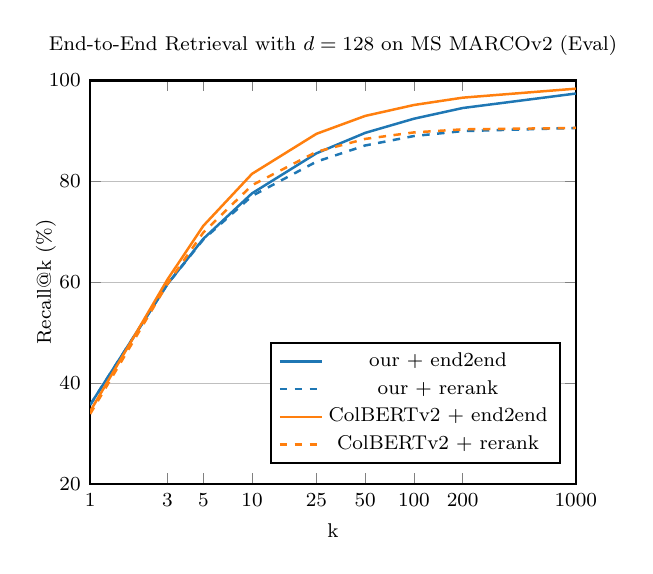
\begin{tikzpicture}[scale=0.9]
        \begin{semilogxaxis}[
            title = {End-to-End Retrieval with $d = 128$ on MS MARCOv2 (Eval)},
            xlabel = {k},
            ylabel={Recall@k (\%)},
            xmin = 1, xmax = 1000,
            ymin = 20, ymax = 100,
            xtick=data,
            xticklabels={1,3,5,10,25,50,100,200,1000},
            ytick = {20, 40, 60, 80, 100},
            legend pos = south east,
            line width = 1pt,
            ymajorgrids = true,
            font=\footnotesize,
            ylabel style={yshift=-1em}, % Reduce the padding between y-axis label and y-axis
            legend style={yshift=0.3em}, % Reduce the padding between legend and plot area
            ]
        
        \addplot[color=plt_blue, line width=1pt]
            coordinates {
            (1, 35.683)(3, 59.577)(5, 68.586)(10, 77.607)(25, 85.544)(50, 89.592)(100, 92.401)(200, 94.519)(1000, 97.393)
        }; \addlegendentry{our + end2end}
        
        \addplot[color=plt_blue, line width=1pt, dashed]
            coordinates {
            (1, 35.649)(3, 59.572)(5, 68.45)(10, 77.088)(25, 83.888)(50, 87.094)(100, 88.964)(200, 89.95)(1000, 90.566)
        }; \addlegendentry{our + rerank}
        
        
        \addplot[color=plt_orange, line width=1pt]
            coordinates {
            (1, 34.373)(3, 60.493)(5, 71.157)(10, 81.475)(25, 89.406)(50, 92.954)(100, 95.119)(200, 96.573)(1000, 98.356)
        }; \addlegendentry{ColBERTv2 + end2end}
        
        \addplot[color=plt_orange, line width=1pt, dashed]
            coordinates {
            (1, 33.864)(3, 59.635)(5, 69.842)(10, 79.216)(25, 85.836)(50, 88.396)(100, 89.685)(200, 90.296)(1000, 90.566)
        }; \addlegendentry{ColBERTv2 + rerank}
        
        \end{semilogxaxis}
    \end{tikzpicture}
    \caption{Comparison between our ColBERT implementation and the official ColBERTv2 checkpoint}
    \label{our-vs-colbertv2} 
\end{figure}
\section{Constant Settings for Neural Model Training and Hyperparameter Search}
\label{appendix:constsettings}
Throughout the training runs, we maintained a batch size $B$ of 42 on MS MARCOv2 and 128 on FANDOM-QA, a dropout rate of 0.1, and utilized the AdamW optimizer with a learning rate of  3e-6. Additionally, we employed linear warmup of the learning rate during the first epoch. We increased the value of $N_d$ to 320 compared to the official ColBERTv2 checkpoint, which used 180. Automatic mixed precision was applied during training and retrieval, with the embeddings being stored with 16-bit precision.
\\
The hyperparameter search was performed only on MS MARCOv2, with the only difference being the use of a smaller batch size of 28 and a higher learning rate of 5e-6.



\section{Hardware specification}
\label{appendix:hardware}
The training of every model was conducted on a single NVidia A100 GPU with 40GB of memory, which was made available through the High-Performance Computing (HPC) infrastructure provided by the ZIH (TU Dresden). 
\\
Training time had great variety, every trained model took 3 to 6 epochs to converge. The training of the preadapted models took about 12 to 18 hours. Fine-tuning on the FANDOM-QA dataset was done in under an hour, and on the Harry Potter dataset after mere minutes.

\section{Similarity Measures}
\label{appendix:similarity}
We tested two differente similarity meassures \\ \\
(1) \textit{cosine similarity}:
$$
sim_{cos}(E_{q_i}, E_{d_j}) := \frac{E_{q_i}^{T}E_{d_j} }{\| E_{q_i} \|\| E_{d_j} \|} 
$$ \\
(2) \textit{negated squared L2-norm} with an optional normalization of the embedding vectors beforehand:
$$
sim_{L2}(E_{q_i}, E_{d_j}) := -{\| E_{q_i} -E_{d_j} \|}^2
$$
$$
sim_{L2,norm}(E_{q_i}, E_{d_j}) := -{\| \frac{E_{q_i}}{\| E_{q_i} \|}  - \frac{E_{d_j}}{\| E_{d_j} \|} \|}^2
$$

\section{Contribution of Contextual-Aware Embeddings}
\label{chap:context}
\begin{figure}
    \centering
    \caption{End-to-End Retrieval Performance of Different Embedding Methods on MS MARCOv1}
    \label{embeddings-plot}
    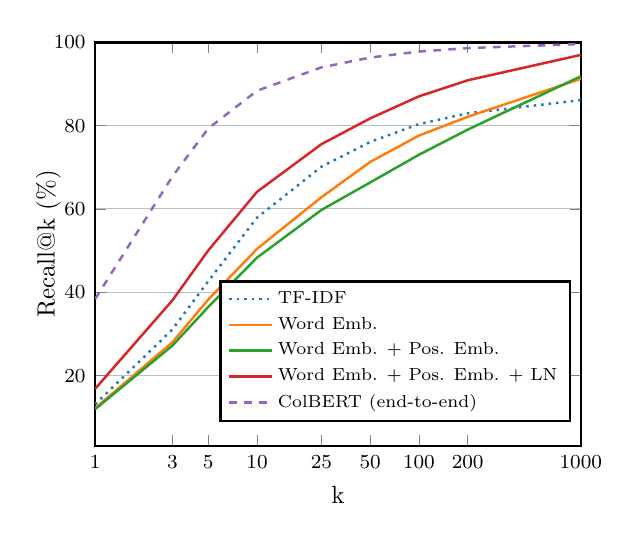
\begin{tikzpicture}[scale = 0.9]
        \begin{semilogxaxis}[
            xlabel={k},
            ylabel={Recall@k (\%)},
            legend style={at={(0.98,0.12)},
                  anchor=south east,
                  font=\scriptsize},
            ticklabel style={font=\footnotesize},
            ymajorgrids=true,
            xmin = 1, xmax = 1000,
            ymax=100,            
            xtick=data,
            xticklabels={
                1,
                3,
                5,
                10,
                25,
                50,
                100,
                200,
                1000},
            cycle list={
                    {plt_blue, dotted},
                    {plt_orange},
                    {plt_green},
                    {plt_red},
                    {plt_purple, dashed},
            },
            line width=1pt, % Adjust line thickness
            ylabel style={yshift=-1em}, % Reduce the padding between y-axis label and y-axis
            legend style={yshift=-1em}, % Reduce the padding between legend and plot area
            legend cell align=left, % Align legend items horizontally
        ]
        % Approach 1 - TF-IDF
        \addplot+[mark=none, line width=1pt] coordinates {
            (1,13.104)
            (3,31.057)
            (5,42.672)
            (10,57.925)
            (25,70.155)
            (50,76.09)
            (100,80.382)
            (200,82.972)
            (1000,86.132)};
        % Approach 2 - Word Emb.
        \addplot+[mark=none, line width=1pt] coordinates {
            (1,12.172)
            (3,27.988)
            (5,38.266)
            (10,50.43)
            (25,62.826)
            (50,71.301)
            (100,77.624)
            (200,82.133)
            (1000,91.254)};
        % Approach 3 - Word Emb. + Pos. Emb.
        \addplot+[mark=none, line width=1pt] coordinates {
            (1,11.933)
            (3,27.188)
            (5,36.487)
            (10,48.32)
            (25,59.768)
            (50,66.373)
            (100,73.015)
            (200,79.049)
            (1000,91.853)};
        % Approach 4 - Word Emb. + Pos. Emb. + LayerNorm
        \addplot+[mark=none, line width=1pt] coordinates {
            (1,16.822)
            (3,38.059)
            (5,50.051)
            (10,64.128)
            (25,75.561)
            (50,81.753)
            (100,87.041)
            (200,90.892)
            (1000,96.994)};
        % Approach 5 - ColBERT
        \addplot+[mark=none, line width=1pt] coordinates {
            (1,38.382)
            (3,67.795)
            (5,79.337)
            (10,88.39)
            (25,94.004)
            (50,96.357)
            (100,97.799)
            (200,98.631)
            (1000,99.61)};
        \legend{TF-IDF, Word Emb., Word Emb. + Pos. Emb., Word Emb. + Pos. Emb. + LN, ColBERT (end-to-end)}
        \end{semilogxaxis}
    \end{tikzpicture}
\end{figure}

To investigate the importance of the Transformer encoder, we analyzed the learned embeddings of our ColBERT model, which was trained on MS MARCOv2. Due to the large size of the resulting 768-dimensional word embeddings, we performed the evaluation on the smaller MS MARCOv1 dataset. For our testing we removed the transformer backbone and the final linear mapping and used solely the output of the embedding layer for the end-to-end retrieval process. We tested three experimental settings: (A) utilizing only word embeddings, (B) incorporating word embeddings with positional embeddings, and (C) combining word and positional embeddings with LayerNorm. \\
The results, presented in Figure \ref{embeddings-plot}, indicated that employing either word embeddings or word and positional embeddings achieved performance comparable to that of TF-IDF. However, when LayerNorm was also applied, the model slightly outperformed TF-IDF. Nevertheless, when compared to the complete ColBERT model, the exclusive use of context-unaware word embeddings resulted in inferior performance. We therefore suspect that the contextual information encoded in the embeddings by the transformer backbone significantly contributes to the overall performance of ColBERT.


\label{appendix:hyperparameters}
\begin{figure*}
    \centering
    \caption{End-to-End Retrieval performance of experimented models with $k=1000$, $\hat{k}=\frac{k}{\lambda}$ on MS MARCOv2. Unlisted values are identical to those of the base model.}
    \label{hparameter-end2end}
    \resizebox{\textwidth}{!}{
        \begin{tabularx}{1.15\textwidth}{c | c c c c c c c | c c c c}
            \hline
                & Backbone & $d$ & sim & norm & Loss & $N_q$ & ${\lambda}$ & MRR@10 & Rec@1 & Rec@10 & Rec@1000 \\
            \hline
                base & BERT & 128 & cosine & yes & cross-entropy & 32 & 2 & 50.42 & 35.65 & 76.97 & 97.46 \\
            \hline  
                & & 64 & & & & &      & 49.94 & 35.19 & 76.48 & 96.69\\ 
                & & 32 & & & & &        & 48.66 & 34.33 & 74.30 & 95.34\\ 
                & & 24 & & & & &        & 48.56 & 34.29 & 74.23 & 94.86\\   
                & & 16 & & & & &        & 43.84 & 30.97 & 67.30 & 91.63\\
                & & 8 & & & &  &        & 30.66 & 21.56 & 47.77 & 71.54\\
            \hline
                & & & L2 & & &  &       & 47.46 & 33.38 & 72.90 & 96.45\\ 
                & & & L2 & no & & &     & 39.04 & 27.41 & 60.61 & 90.88\\ 
            \hline
                & RoBERTa & & & & & &   & 47.50 & 33.55 & 72.98 & 96.51\\
                & & & & & MSE &     &   & 13.20 & 9.42  & 20.82 & 86.98\\ 
                \textbf{best} & & & & & & \textbf{64}   &   & \textbf{51.11} & \textbf{36.06} & \textbf{78.06} & \textbf{97.43} \\ 
            \hline
                & & & & & & & 1         & 50.42 & 35.65 & 76.96 & 97.40 \\
                & & & & & & & 5         & 50.42 & 35.65 & 76.96 & 97.24\\
                & & & & & & & 10        & 50.41 & 35.65 & 76.93 & 96.29 \\
                & & & & & & & 20        & 50.32 & 35.63 & 76.63 & 93.72 \\
            \hline
        \end{tabularx}
    }
\end{figure*}

\label{appendix:rerank}
\begin{figure*}
    \centering
    \caption{Rerank Retrieval performance of experimented models on MS MARCOv2.
    Unlisted values are identical to those of the base model.}
    \centering
    \label{hparameter-rerank}
    \resizebox{\textwidth}{!}{
        \begin{tabularx}{1.1\textwidth}{c | c c c c c c | c c c c}            
        \hline
            & Backbone & $d$ & Sim & norm & Loss Fun & $N_q$ & MRR@10 & Rec@1 & Rec@10 & Rec@1000 \\
            \hline
            base & BERT & 128 & cosine & yes & cross-entropy & 32 & 50.49 & 35.70 & 76.74 & 90.57\\
            \hline  
                & & 64 & & & &      & 50.10 & 35.28 & 76.48 &  \\ 
                & & 32 & & & &      & 49.47 & 34.86 & 75.57 &  \\ 
                & & 24 & & & &      & 49.48 & 34.83 & 75.62 &  \\   
                & & 16 & & & &      & 47.21 & 33.07 & 72.97 &  \\
                & & 8 & & & &      & 41.65 & 28.59 & 66.67 &  \\
            \hline
                & & & L2 & & &      & 48.50 & 34.06 & 74.33 &  \\ 
                & & & L2 & no & &  & 42.67 & 29.62 & 67.11 &  \\ 
            \hline
                & RoBERTa & & & & & & 49.86 & 35.15 & 76.26 &  \\
                & & & & & MSE    & & 24.42 & 15.89 & 43.20 &  \\ 
                \textbf{best} & & & & & & \textbf{64}    & \textbf{50.91} & \textbf{35.94} & \textbf{77.33} & \textbf{90.57}\\ 
             \hline
        \end{tabularx}
    }
\end{figure*}


\begin{figure*}
    \centering
    \caption{End-to-End Retrieval on The Witcher ($d=24$, $sim=\text{cosine}$)}
    \label{FandomQAvHPonWitcher}
    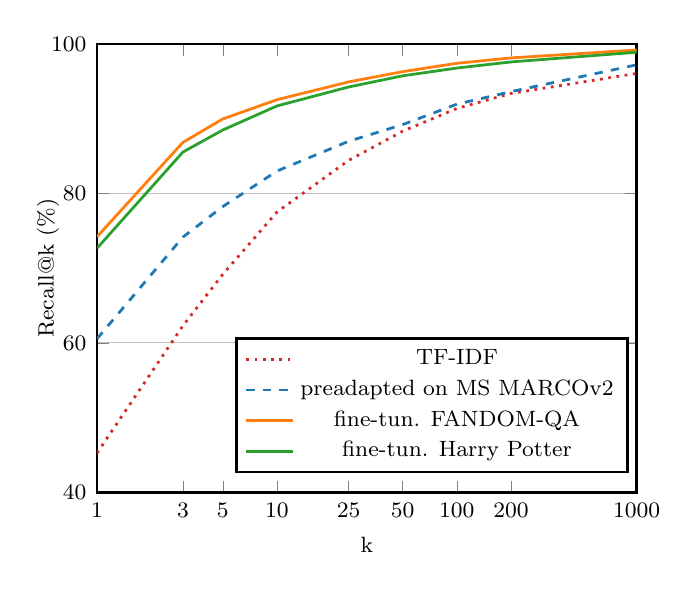
\begin{tikzpicture}
        \begin{semilogxaxis}[
            xlabel = {k},
            ylabel={Recall@k (\%)},
            xmin = 1, xmax = 1000,
            ymin = 40, ymax = 100,
            xtick=data,
            xticklabels={1,3,5,10,25,50,100,200,1000},
            legend pos = south east,
            line width = 1pt,
            ymajorgrids = true,
            font=\footnotesize,
            ylabel style={yshift=-1em}, % Reduce the padding between y-axis label and y-axis
            legend style={yshift=0.2em, xshift=0.3em}, % Reduce the padding between legend and plot area
            ]
            
            \addplot[color=plt_red, line width=1pt, dotted]
                coordinates {
                (1, 45.277)(3, 62.293)(5, 69.183)(10, 77.511)(25, 84.422)(50, 88.336)(100, 91.372)(200, 93.389)(1000, 96.066)
                }; \addlegendentry{TF-IDF}
            
            \addplot[color=plt_blue, line width=1pt, dashed]
                coordinates {
                (1, 60.56)(3, 74.16)(5, 78.25)(10, 83)(25, 86.98)(50, 89.22)(100, 91.95)(200, 93.63)(1000, 97.22)
                }; \addlegendentry{preadapted on MS MARCOv2}
                    
            \addplot[color=plt_orange, line width=1pt]
                coordinates {
                (1, 74.216)(3, 86.838)(5, 89.974)(10, 92.55)(25, 94.927)(50, 96.305)(100, 97.424)(200, 98.143)(1000, 99.201)
                }; \addlegendentry{fine-tun. FANDOM-QA}
                
            \addplot[color=plt_green, line width=1pt]
                coordinates {
                (1, 72.678)(3, 85.54)(5, 88.496)(10, 91.712)(25, 94.248)(50, 95.746)(100, 96.785)(200, 97.603)(1000, 98.902)
                }; \addlegendentry{fine-tun. Harry Potter}
                
        \end{semilogxaxis}
    \end{tikzpicture}
\end{figure*}


\begin{figure*}[h]
    \begin{center}
    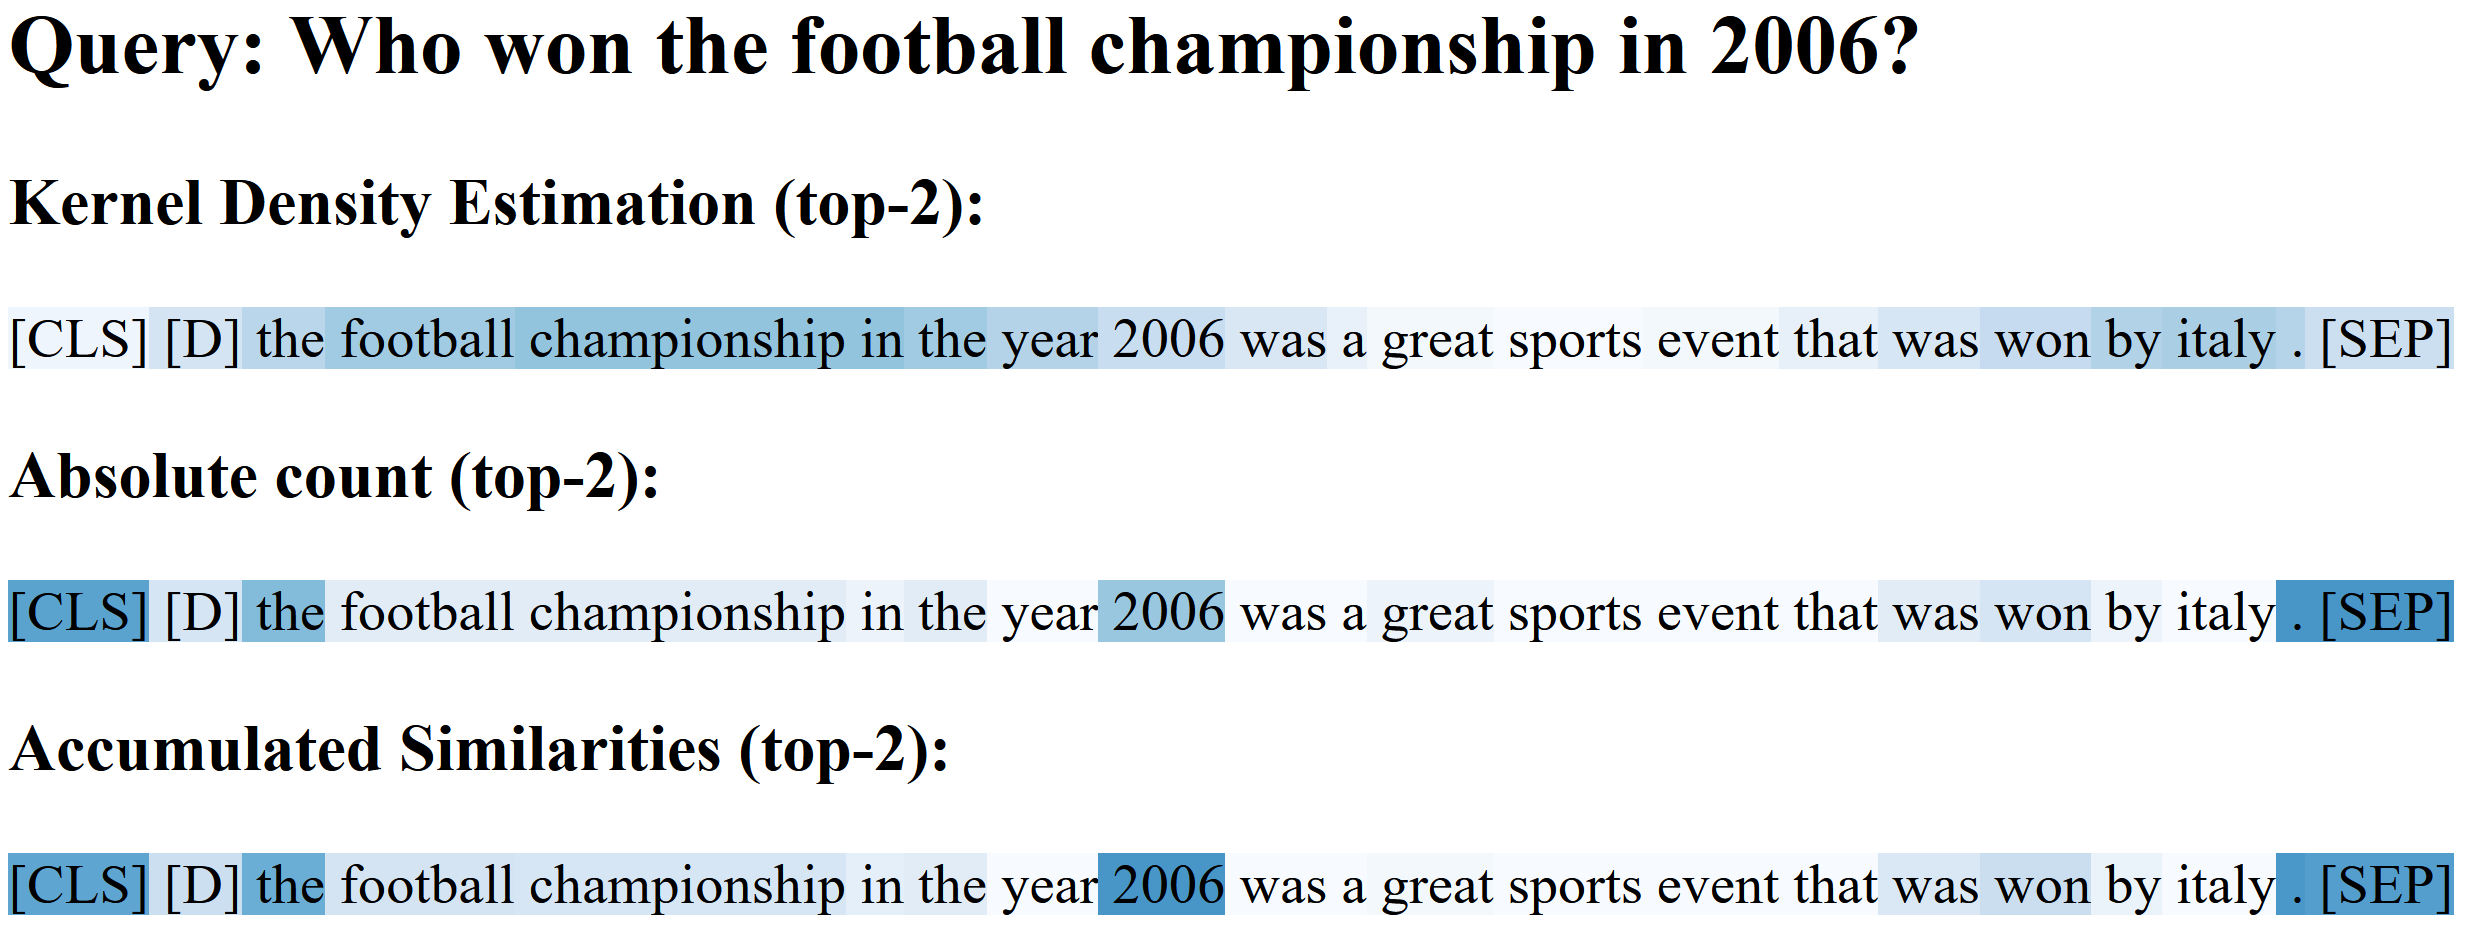
\includegraphics[width=1.0\textwidth]{"./images/heatmap1.png"}
    \end{center}
    \caption{KDE, Abs. Count, Acc. Similarities - ColBERTv2 }
    \small
    \center Custom Query and Passage
    \label{fig:example1}
\end{figure*}

\begin{figure*}[h]
    \begin{center}
    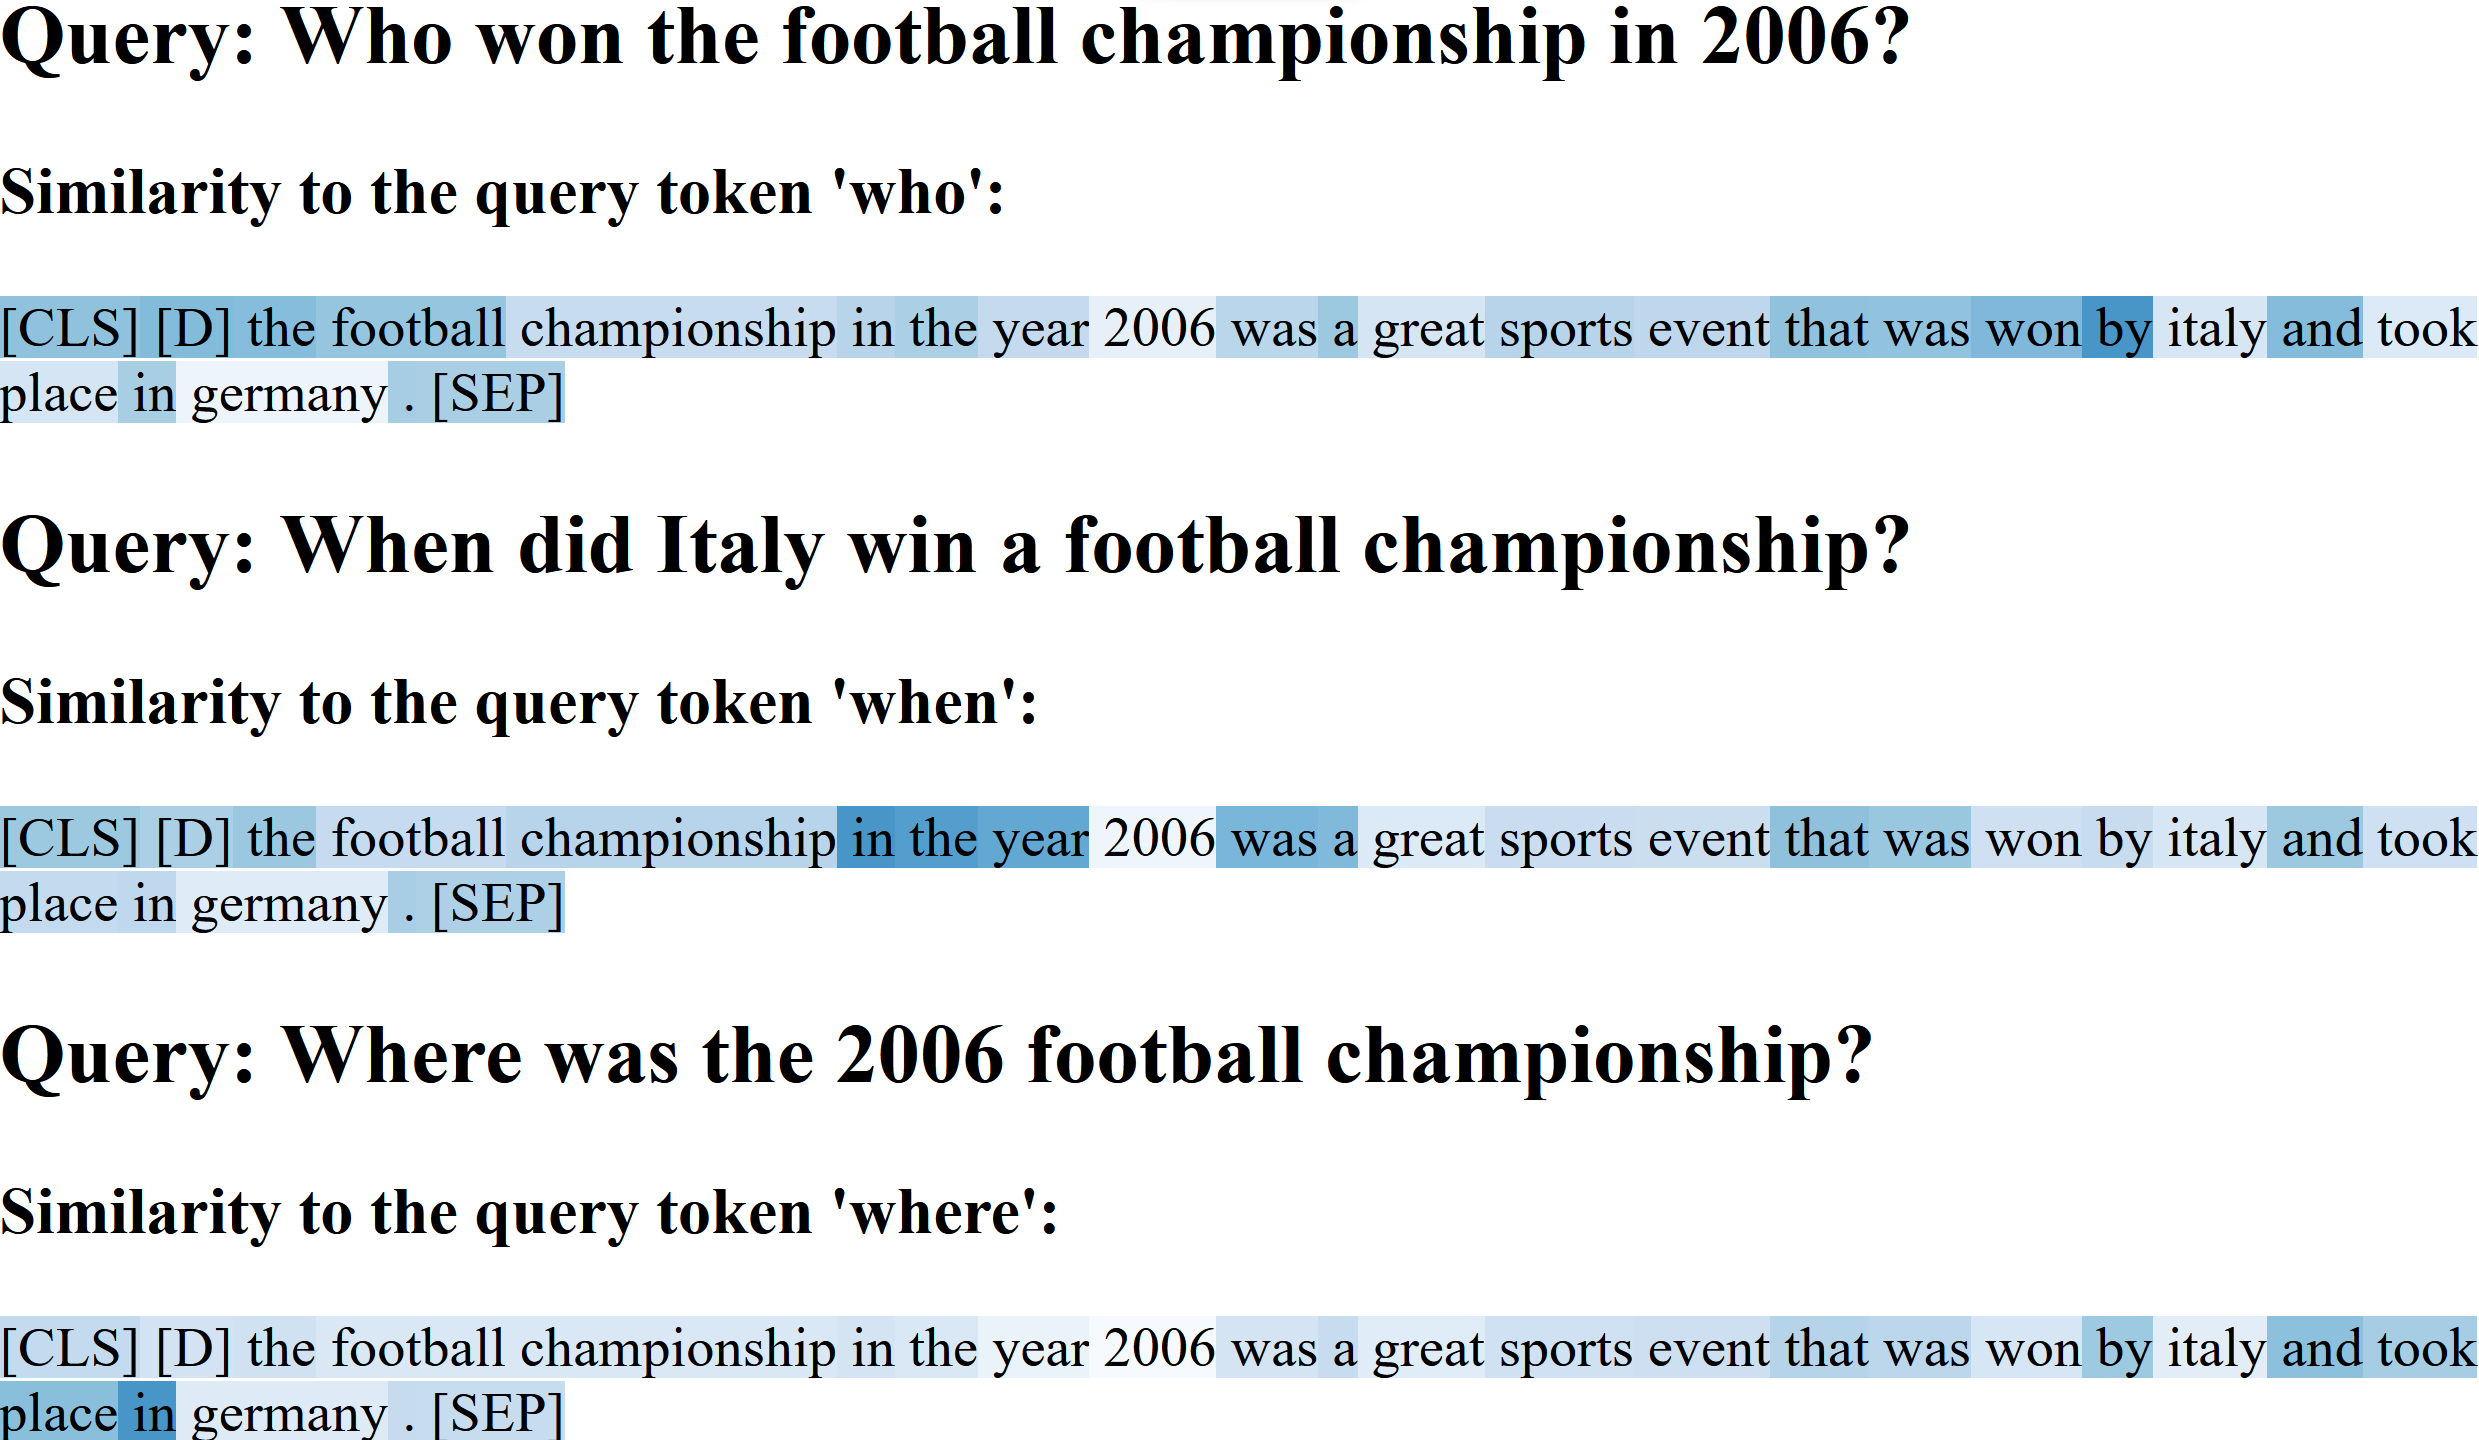
\includegraphics[width=1.0\textwidth]{"./images/first_word_heatmap.png"}
    \end{center}
    \caption{Single Token Similarity - ColBERTv2 }
    \small
    \center Custom Query and Passage
    \label{fig:example2}
\end{figure*}

\begin{figure*}[h]
    \begin{center}
    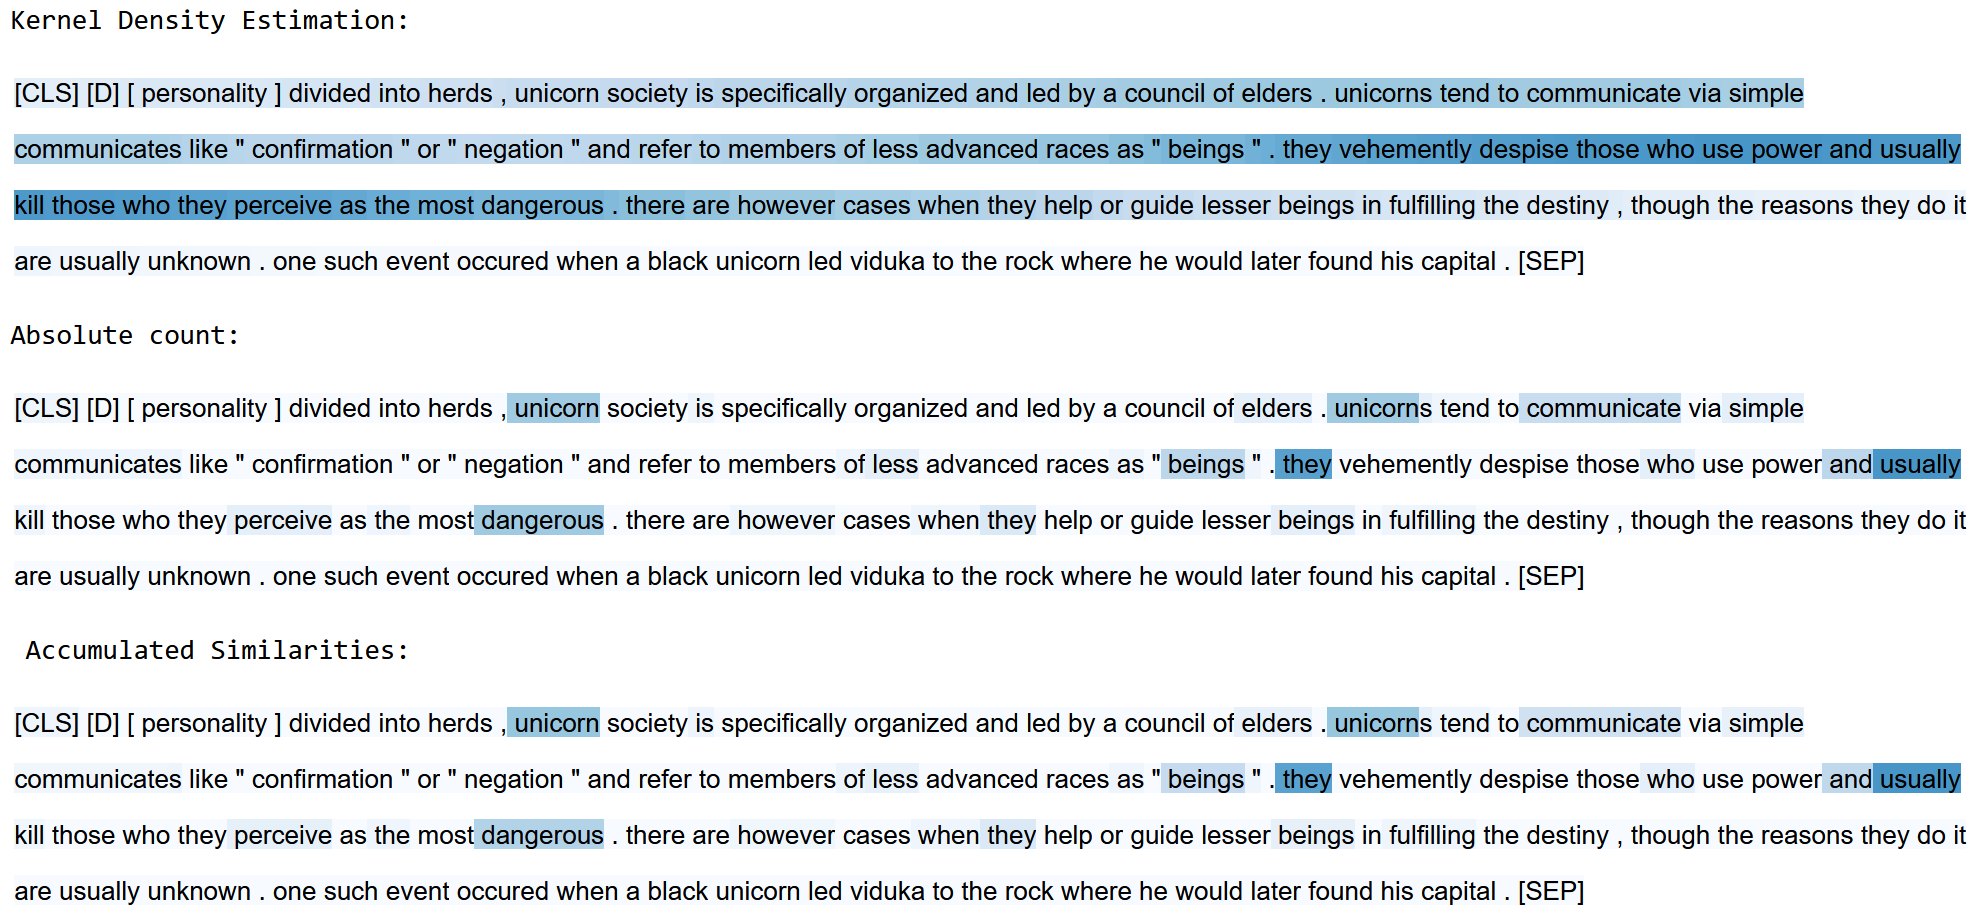
\includegraphics[width=1.0\textwidth]{"./images/unicorns.png"}
    \end{center}
    \caption{End-to-end Retrieval - ColBERTv2 - 24 dimensional embedding}
    \small
    \center Custom Query: Are unicorns peaceful or do they harm others?, Top 1 Passage retrieved from \href{https://witcher.fandom.com}{Witcher Fandom}
    \label{fig:example3}
\end{figure*}

\begin{figure*}[h]
    \begin{center}
    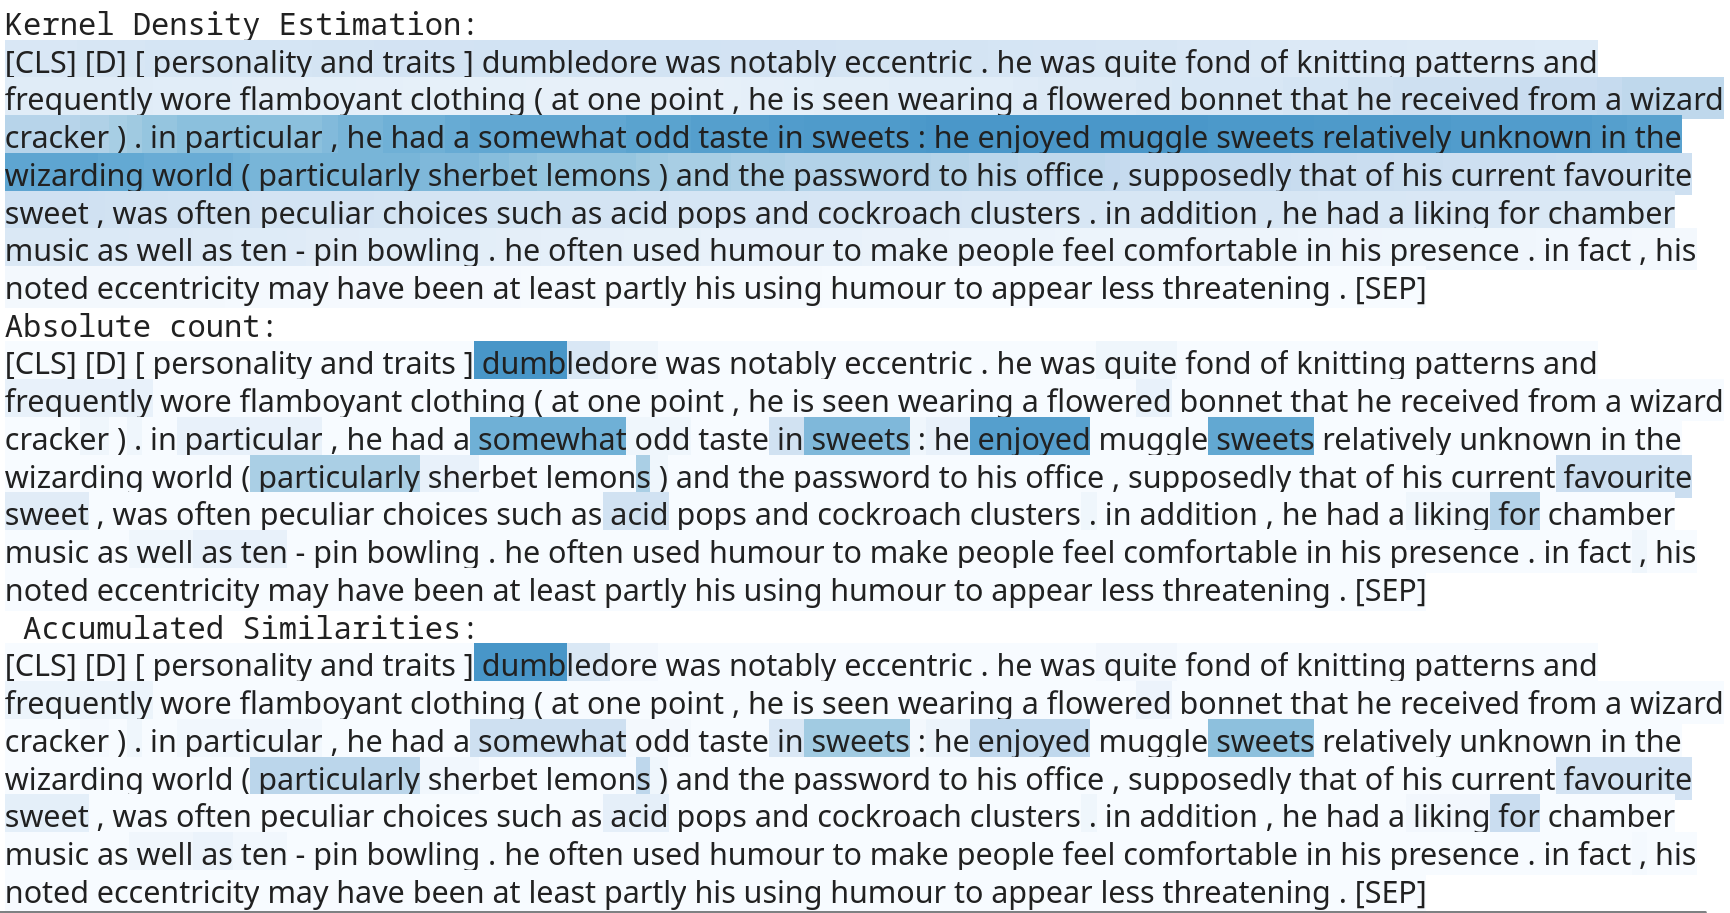
\includegraphics[width=1.0\textwidth]{"./images/sweets.png"}
    \end{center}
    \caption{End-to-end Retrieval - ColBERT preadapted MS MARCOv2, fine-tuned on Harry Potter - 24 dimensional embedding}
    \small
    \center Custom Query: What is Dumbledore's favourite candy?, Top 1 Passage retrieved from \href{https://harrypotter.fandom.com}{Harry Potter Fandom}
    \label{fig:example4}
\end{figure*}


\begin{figure*}[ht]
    \centering
    \caption{Random Samples out of the FANDOM-QA Dataset. Each passage has two positive and two negative queries.}
    \label{tab:fandom-qa}
    \begin{tabular}{|p{4.5cm}|p{4.5cm}|p{4.5cm}|}
        \hline
        \textbf{Passage} & \textbf{Positive Queries} & \textbf{Negative Queries} \\
        \hline
        Sincantar is an Altmer mystic and a member of the Mages Guild residing in Marbruk, Greenshade. He is found at the local branch, selling his wares. &
        1. Who is Sincantar and where does he live? \linebreak \linebreak 2. What is Sincantar's occupation and where can he be found?&
        1. What type of mystical abilities does Sincantar possess? \linebreak \linebreak 2. How long has Sincantar been a member of the Mages Guild?\\
        \hline
        [Lions in the wizarding world] It was a possible corporeal form of the Patronus Charm. Patricia Rakepick's Patronus took the form of a lioness. &
        1. What is one possible corporeal form of the Patronus Charm in the wizarding world? \linebreak \linebreak 2. Whose Patronus took the form of a lioness according to the given paragraph?&
        1. Are there any other characters besides Patricia Rakepick whose Patronus takes the form of a lioness? \linebreak \linebreak 2. Why do some witches and wizards choose a lion as their Patronus?\\
        \hline
        [Chest] Usually the largest storage containers found and they normally contain items of higher value than other containers. Chests can vary in appearance depending on their location. As chests are the ''best'' containers available, the term ''chest'' is often used for any storage container found within a dungeon. Chests may be locked or trapped, but never both. The one exception is the locked and trapped chest inside Pinewatch, in the room with the Unusual Gem. &
        1. What is the difference between chests and other storage containers in a dungeon? \linebreak \linebreak 2. Can a chest be both locked and trapped? &
        1. What is the highest value item found in a chest?  \linebreak \linebreak 2. What are the different appearances of chests in different locations?\\
        \hline
    \end{tabular}
\end{figure*}


\begin{figure*}
    \centering
    \caption{Dataset sizes and median count of words in a Passage or Query}
    \label{table1}
    \setlength{\tabcolsep}{4pt} % Reduce cell padding
    \begin{tabular}{ccccc}
    \hline
    \textbf{Dataset} & \textbf{\# Passages} & \textbf{\# Queries} & \multicolumn{2}{c}{\textbf{Median word count}} \\
    & & & \textbf{Passage} & \textbf{Query} \\
    \hline

    \texttt{MS MARCO v1} & 707,946 & 92,373 & 72 & 6 \\
    \texttt{MS MARCO v2} & 8,132,834 & 909,824 & 50 & 6 \\
    \hline
    \texttt{FANDOM-QA} & 705,136 & 576,526 & 53 & 11 \\
    \hline
    \end{tabular}
\end{figure*}





\end{document}
